\documentclass[10pt,twocolumn,letterpaper]{article}

\usepackage{cvpr}
\usepackage{times}
\usepackage{epsfig}
\usepackage{graphicx}
\usepackage{amsmath}
\usepackage{amssymb}

\cvprfinalcopy

\def\cvprPaperID{****}
\def\httilde{\mbox{\tt\raisebox{-.5ex}{\symbol{126}}}}

% Pages are numbered in submission mode, and unnumbered in camera-ready
\ifcvprfinal\pagestyle{empty}\fi
\begin{document}

%%%%%%%%% TITLE
\title{M5 Forecasting - Accuracy: Estimate the unit sales of Walmart retail goods}

\author{Flavio Amurrio-Moya\\
George Mason University\\
4400 University Dr, Fairfax, VA 22030\\
{\tt\small famurrio@gmu.edu}
\and
Pyoung Kang Kim\\
George Mason University\\
4400 University Dr, Fairfax, VA 22030\\
{\tt\small pkim23@gmu.edu}
}

\maketitle
\thispagestyle{empty}

%%%%%%%%% ABSTRACT
\begin{abstract}
% Problem, gap, approach, key results
   The ``M5 Forecasting - Accuracy: Estimate the unit sales of Walmart retail
   goods'' competition (will be referred as the ``M5 Forecasting Competition''
   and ``The Competition'') challenged Kaggle users to design a learning model
   that would be able to predict how many of a certain item would be sold
   on a given day. In this paper we embark in the challenge to create such a
   model and improve on current strategies.
\end{abstract}

%%%%%%%%% BODY TEXT
\section{Introduction}
% Broad problem and impact
% scientific gap(what technical aspects have not yet been solved)
% summary approach (should include reference to technical gap)
% key results

The introduction goes here.


%-------------------------------------------------------------------------
\section{Approach}
% Background tutorial (if necessary)
% Your technical innovation (might be multiple pages/sections, with repeated reference to scientific gap)
The Approach goes here.

%-------------------------------------------------------------------------
\section{Results}
% Data sets, simulator, implementation details
% Empirical results (might be multiple pages)
The results get explained here.

%-------------------------------------------------------------------------
\section{Related Work}
% Dont just say whats been done. Point out how prior work relates to yours and to the scientific gap you set forth in the intro.
The relate work goes here

%-------------------------------------------------------------------------
\section{Summary/Discussion/Conclusion}
% Summary problem, approach, result, in past tense
% Discuss open questions, promising research directions
The Summary Goes here

%-------------------------------------------------------------------------
\section{References}
The References Goes here









%-------------------------------------------------------------------------
\section{\LaTeX\ Reference Section}
\verb'\cvprfinalcopy' Is for different font

(e.g.\ this line is $095.5$)

An example of a bad paper:
\begin{quote}
\begin{center}
    An analysis of the frobnicatable foo filter.
\end{center}

   In this paper we present a performance analysis of our
   previous paper [1], and show it to be inferior to all
   previously known methods.  Why the previous paper was
   accepted without this analysis is beyond me.

   [1] Removed for blind review
\end{quote}

This is how you cite a reference submission~\cite{Authors06} as additional material and

\begin{quote}
and this is a quote and a another special formatting {\tt eccv06.pdf}.
\end{quote}

{\em require} more special formatting

``Zero-g frobnication: How being the only people in the world with access to
the Apollo lander source code makes us a wow at parties'', by Zeus \etal.

FAQ: Are acknowledgements OK?  No.  Leave them for the final copy.


\begin{figure}[t]
  \begin{center}
    \fbox{\rule{0pt}{2in} \rule{0.9\linewidth}{0pt}}
    % 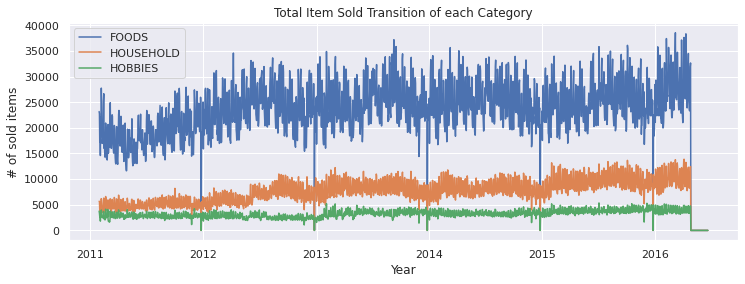
\includegraphics[width=0.8\linewidth]{img/meh.png}
  \end{center}
    \caption{Example of caption.  It is set in Roman so that mathematics
    (always set in Roman: $B \sin A = A \sin B$) may be included without an
    ugly clash.}
  \label{fig:long}
  \label{fig:onecol}
\end{figure}

\noindent
Compare the following:\\
\begin{tabular}{ll}
 \verb'$conf_a$' &  $conf_a$ \\
 \verb'$\mathit{conf}_a$' & $\mathit{conf}_a$
\end{tabular}\\
See The \TeX book, p165.

The space after \eg, meaning ``for example'', should not be a
sentence-ending space. So \eg is correct, {\em e.g.} is not.  The provided
\verb'\eg' macro takes care of this.

When citing a multi-author paper, you may save space by using ``et alia'',
shortened to ``\etal'' (not ``{\em et.\ al.}'' as ``{\em et}'' is a complete word.)

For this citation style, keep multiple citations in numerical (not
chronological) order, so prefer \cite{Alpher03,Alpher02,Authors06} to
\cite{Alpher02,Alpher03,Authors06}.


\begin{figure*}
  \begin{center}
    % \fbox{\rule{0pt}{2in} \rule{.9\linewidth}{0pt}}
    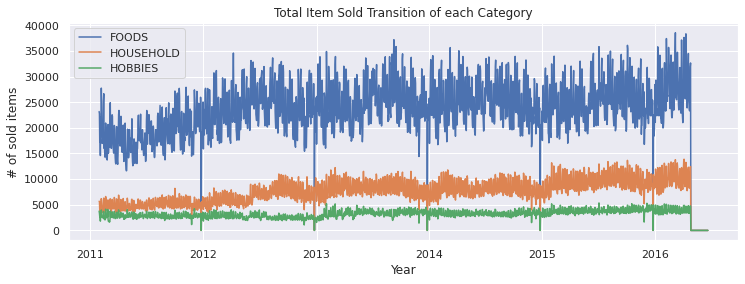
\includegraphics[width=0.8\linewidth]{img/totalItemSoldofEachCategory.png}
  \end{center}
    \caption{Total items sold of each category.}
  \label{fig:short}
\end{figure*}

\begin{figure*}
  \begin{center}
    % \fbox{\rule{0pt}{2in} \rule{.9\linewidth}{0pt}}
    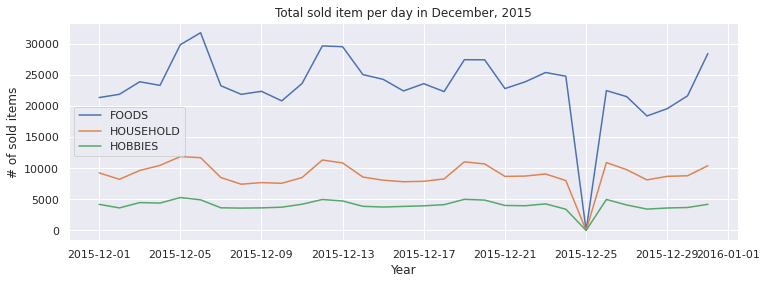
\includegraphics[width=0.8\linewidth]{img/totalSoldItemPerDayDec2015.png}
  \end{center}
    \caption{Total items sold per day in December 2015.}
  \label{fig:short}
\end{figure*}

\begin{figure*}
  \begin{center}
    % \fbox{\rule{0pt}{2in} \rule{.9\linewidth}{0pt}}
    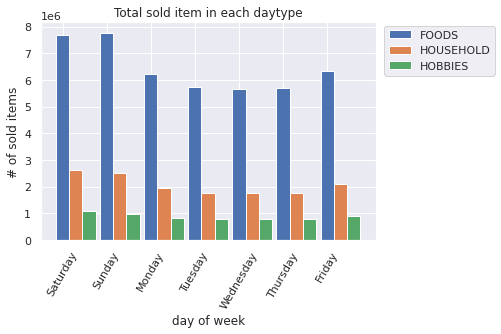
\includegraphics[width=0.8\linewidth]{img/totalSoldItemInEachDayOfWeek.png}
  \end{center}
    \caption{Total items sold each day of the week}
  \label{fig:short}
\end{figure*}

\begin{figure*}
  \begin{center}
    % \fbox{\rule{0pt}{2in} \rule{.9\linewidth}{0pt}}
    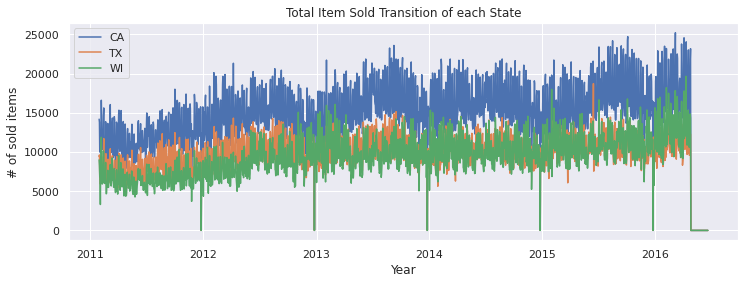
\includegraphics[width=0.8\linewidth]{img/totalItemSoldInEachState.png}
  \end{center}
    \caption{Total items sold in each state.}
  \label{fig:short}
\end{figure*}


This is fractions text area is $6\frac78$ inches (17.5 cm) wide by $8\frac78$
and more $\frac{5}{16}$ and other $8.5 \times 11$-inch

Reference figurers Figures~\ref{fig:onecol} and~\ref{fig:short}.  Short captions should be centred.

\noindent For no indent

FIRST-ORDER HEADINGS. (For example, {\large \bf 1. Introduction})

SECOND-ORDER HEADINGS. (For example, { \bf 1.1. Database elements})

Please use footnotes\footnote {This is what a footnote looks like.  It
often distracts the reader from the main flow of the argument.} sparingly.

\begin{table}
  \begin{center}
    \begin{tabular}{|l|c|}
      \hline
      Method & Frobnability \\
      \hline\hline
      Theirs & Frumpy \\
      Yours & Frobbly \\
      Ours & Makes one's heart Frob\\
      \hline
    \end{tabular}
  \end{center}
  \caption{Results.   Ours is better.}
\end{table}

When placing figures in \LaTeX, it's almost always best to use
\verb+\includegraphics+, and to specify the  figure width as a multiple of
the line width as in the example below
{\small\begin{verbatim}
   \usepackage[dvips]{graphicx} ...
   \includegraphics[width=0.8\linewidth]
                   {myfile.eps}
\end{verbatim}
}


{\small
\bibliographystyle{ieee}
\bibliography{egbib}
}

\end{document}
